%
%Independent Study Template.
% School of Computing
% University of Colorado at Colorado Springs
%
\documentclass[10pt]{proposal}
%\usepackage{times}
\usepackage[small,compact]{titlesec}
\usepackage[small,it]{caption}
\usepackage{url}
 \usepackage{hyperref} 
 \hypersetup{breaklinks} 
 \usepackage{graphicx}
 \usepackage{xcolor}
\usepackage{amssymb}
\usepackage{longtable}
\usepackage{pdflscape}
\usepackage{array}
\usepackage{blindtext}
\usepackage{titlesec}


% This is nice for source code listings
% \usepackage{listings}

% This is needed to include figures
\usepackage{graphicx}
\usepackage{sidecap}

% Use any additional packages you might need


%
% Give values to the variables used in this document
%

\title{Low Level Driver Test Tool}
\department{Department of Computer Science\\ at the University of Colorado at Colorado Springs\\ School of Engineering and Applied Science}
\documenttype{Masters Project Proposal}
\major{Software Engineering }
\proposalday{10}
\proposalmonth{Mar}
\proposalyear{2015}
\author{Poorani Dharmasivam}
\committeechair{Dr. Kristen Walcott Justice, Advisor}
 \committeememberfour{Dr. Al Glock}
 \committeememberfive{Dr. Jia Rao}
 \committeemembersix{}


%
% PDF Setup -- You should not  change this
%
\hypersetup{
    colorlinks,
    linkcolor={black},
    citecolor={black},
    filecolor={black},
    urlcolor={black},
    pdftitle={\thetitle},
    pdfauthor={\theauthor},
    pdfsubject={\thedocumenttype},
    pdfkeywords={University of Colorado at Colorado Springs, \theauthor, \thedocumenttype},
    pdfstartpage={1}
}


%
% User-specified command definitions/redefinitions
%
%\newcommand{\cplusplus}{{\rm C\raise.5ex\hbox{\small ++}}}
%\setcounter{secnumdepth}{5}
%\setcounter{tocdepth}{5}

%\makeatletter
%\renewcommand\paragraph{%
%   \@startsection{paragraph}{4}{0mm}%
%      {-\baselineskip}%
%      {.5\baselineskip}%
%      {\normalfont\normalsize\bfseries}}
%\makeatother
\usepackage{wrapfig}

\newcommand{\squishlist}{
 \begin{list}{$\bullet$}
  { \setlength{\itemsep}{0pt}
     \setlength{\parsep}{3pt}
     \setlength{\topsep}{3pt}
     \setlength{\partopsep}{0pt}
     \setlength{\leftmargin}{1.5em}
     \setlength{\labelwidth}{1em}
     \setlength{\labelsep}{0.5em} } }

\newcommand{\squishlisttwo}{
 \begin{list}{$\bullet$}
  { \setlength{\itemsep}{0pt}
     \setlength{\parsep}{0pt}
    \setlength{\topsep}{0pt}
    \setlength{\partopsep}{0pt}
    \setlength{\leftmargin}{2em}
    \setlength{\labelwidth}{1.5em}
    \setlength{\labelsep}{0.5em} } }

\newcommand{\squishend}{
  \end{list}  }


\begin{document}
	
%   ==========================================================================
%   Begin front matter (pages are numbered with roman numerals)
%   ==========================================================================
     \begin{frontmatter}
       \maketitle
        %\tableofcontents
       \newpage

        % Generate the abstract	

        \textbf{Abstract}\vspace{3 mm}

In Linux Kernel, the SCSI storage drivers are maintained as three different levels, the high level drivers handles device specific code, the middle level is a core layer which provides the primary functionality of the SCSI subsystem and the Low Level Drivers (LLD) which contains hardware specific code. Since the LLD are hardware specific, they are predominantly developed by hardware vendors whereas the Upper Level and Middle Level drivers are mostly implemented by the open source developers who are responsible for the SCSI subsystem maintenance.

Since the LLD are developed by developers from vast number of hardware vendor organization, the LLD are highly error prone compare to other part of the SCSI stack.  There was no tool available for the developers to verify the functionality of LLD at unit level as most of the unit test frameworks are currently available only for user space applications.  

This paper presents a tool which assist LLD developers to verify the code at individual function level.  The tool is implemented as a kernel module with a helper application. The developers of LLD need to modify their code to register the LLD interfaces with LLD tester and the LLD tester will execute the interfaces with many possible input parameters and provide a report on what tests are passed and what are failed.   The LLD tester tool is executed against the sample LLD for RAM disk provided as part of Linux kernel and on XYZ driver and captured N number of errors.



               \end{frontmatter}
       
              
 \newpage    
\renewcommand*\contentsname{Contents}           
\tableofcontents{}
\newpage    


%   ==========================================================================
%   Begin main matter (pages are numbered with arabic numerals)
%   ==========================================================================
    \singlespacing     % Text should be double spaced
    \pagestyle{fancy}  % Turn the nice header on for the rest of the document

     
% Cite the software repositories

\section{Introduction}\vspace{3 mm}

There are many tools available to ease the unit testing process. Cunit is a unit testing framework for C [Ref] is a tool which aids unit testing of C applications.  The CuTest [Ref] is another tool which is also used for unit testing C applications. The unit test tools provide library functions for the developers or testers to create a test suit and add test cases to it. The test tool library can be statically linked to the unit. These types of unit test tools provide a system for writing, administering, and running unit tests in C. These typically are built as a static library which is linked with the testing code. CUnit uses a simple framework for building test structures, and provides a rich set of assertions for testing common data types. In addition, several different interfaces are provided for running tests and reporting results. These include automated interfaces for code controlled testing and reporting, as well as interactive interfaces allowing the user to run tests and view results dynamically. A CUnit ``test"  is a C function having the signature ``void test\_func(void)". There are no restrictions on the content of a test function, except that it should not modify the CUnit framework.  A test function may call other functions (which also may not modify the framework). Registering a test will cause its function to be run when the test is run. \\

An example test function for a routine that returns the maximum of 2 integers might look like: \\

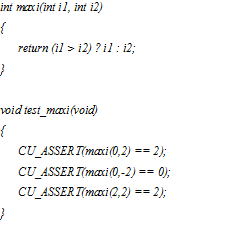
\includegraphics[scale=1]
{fig4}


CUnit provides a set of assertions for testing logical conditions.  The success or failure of these assertions is tracked by the framework, and can be viewed when a test run is complete. Each assertion tests a single logical condition, and fails if the condition evaluates to FALSE. Upon failure, the test function continues unless the user chooses the `xxx\_FATAL'  version of an assertion. In that case, the test function is aborted and returns immediately.  \\

However all of the unit test tools for C are available for user space application programs. There are some kernel specific limitations which prevent development of a generic unit testing framework for Linux kernel modules.  Few of the complexities of testing a kernel code (a device driver functions or a kernel module functions)  using a standard unit test tools like Cunit or CuTest are listed below.\\
\begin{itemize}
\item Unit testing kernel level code using the standard tool is highly impossible. Either the tool has to be ported into a kernel module so that it can access the kernel code at unit level or the kernel code has to be moved to user space, but moving the kernel code to user space is not possible due to the strong dependency between the kernel APIs. For example the memory allocation is done in kernel code using the function kmalloc() but whereas the same is done at user space using malloc().\\

\item Unit testing from user space using general applications doesn’t solve the purpose.  For example, if a function in a kernel module needs to be verified, then a particular application level call which executes the particular kernel modules function after passing through many kernel layers need to be identified and executed. But this doesn’t solve the primary purpose of unit testing. A new method is required to directly invoke the kernel function with proper prerequisites setup so the kernel function alone can be executed with varying arguments to the same. 
\item  Even if the unit test tools like C-Unit or CUTest are ported to kernel space, the test cases cannot be executed directly from a kernel module as the execution of test code requires either a user level process context or a specific kernel thread.  Developing either of them for individual modules is costly and will consume majority of testing resources.
\item  The kernel modules have high level of interactions with them so applying a generic method without knowing the internal communication between kernel modules may not yield a proper test tool.

\end{itemize}



     
\section{Background}\vspace{3 mm}
\subsection{Unit Testing}
Unit testing is important part of software development. Unit testing is a software testing method that seeks to uncover new software bugs hidden at individual units of the software and it will be the first pass of testing as soon as individual building blocks of a big software is build.  Unit testing is a method by which individual units of source code, sets of one or more computer program modules together with associated control data, usage procedures, and operating procedures are tested to determine if they are fit for use.\\

There are many tools available to ease the unit testing process. Cunit a unit testing framework for C [1] is a tool which aids unit testing of C applications.  The CuTest [2] is another tool which is also used for unit testing C applications.\\

\subsection{SCSI}

SCSI (Acronym for Small Computer System Interface) is a collection of ANSI standards and proposed standards which define I/O busses primarily intended for connecting storage subsystems or devices to hosts through host bus adapters. Originally intended primarily for use with small (desktop and desk-side workstations) computers, SCSI has been extended to serve most computing needs, and is arguably the most widely implemented I/O control structure in use today.  SCSI Architecture Model (SAM) is an ANSI standard that defines the generic requirements and overall framework in which other SCSI standards are defined. \\

The first two SCSI standards (SCSI and SCSI-2) were all-in-one standards. They included everything from cables and connectors to protocols to command sets in one standard. The InterNational Committee for Information Technology Standards (INCITS) T10 Technical adopted a layered standards approach much like the International Organization for Standardization (ISO) Reference Model for networking standards. This approach divides SCSI into multiple layers of standards. The lowest layer deals with physical interfaces (also called transports). The next layer up deals with transport protocols usually directly associated with one physical transport standard. The top layer consists of command sets associated with specific devices such as disk drives or tape drives. \\

The image mentioned below is reproduced from T10 SAM specification depicts how the different standards of SCSI are layered in the SAM.  From the picture below, it can be seen that majority of the storage devices, whether  it is SAS, SATA, SCSI, FC,  iSCSI or the latest PCIe all are covered under the big umbrella of SCSI.\\

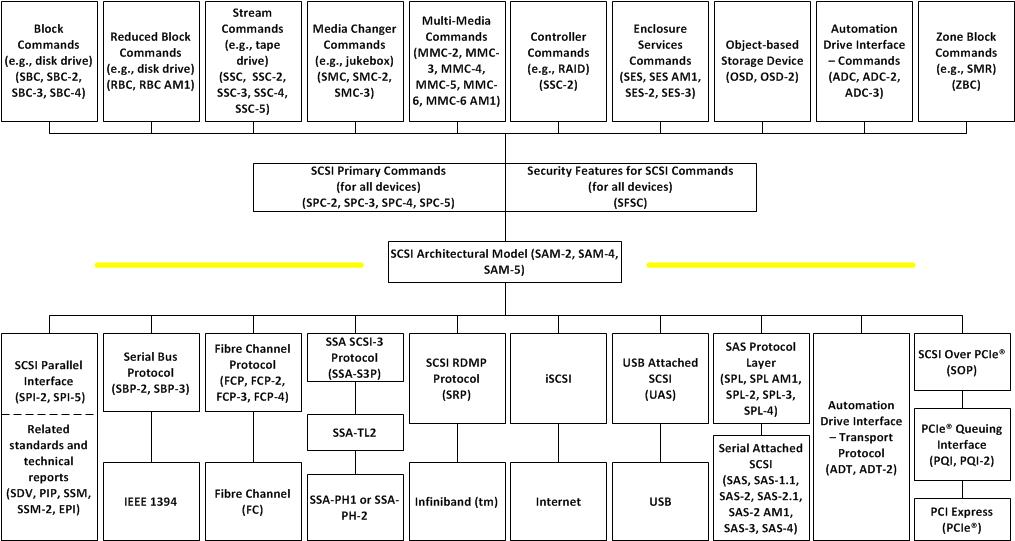
\includegraphics[scale=.6]
{SAM}

\subsection{Linux Kernel’s SCSI Device Driver Architecture} 

Layered SCSI architecture is mirrored in the software architecture as well. Operating systems use layered driver structures such as SCSI Common Access Method (CAM). This architecture has one or more class drivers that share one or more host bus adapter drivers. This allows both disk drives and tape drives to coexist on the same parallel SCSI bus. It also permits a disk class driver to control both parallel SCSI and Fiber Channel disk drives. This protects software investment as people migrate to newer physical interfaces.\\

The Linux kernel I/O subsystem consists of multiple layers of drivers.  The SCSI subsystem is part of the Linux I/O subsystem and handles majority of storage devices belong to different storage protocol family.  The Parallel SCSI (SPI), Fibre Channel (FC), Serial Attached Scsi (SAS) and Serial ATA (SATA) devices are managed by the SCSI subsystem of Linux kernel.   The SCSI subsystem is a layer between the File System Drivers and actual storage Host Bus Adapter (HBA) hardware. The SCSI subsystem itself is a layered architecture with three different layers of drivers (or kernel modules). The architecture of the I/O subsystem and SCSI subsystem are represented in the pictures below.\\

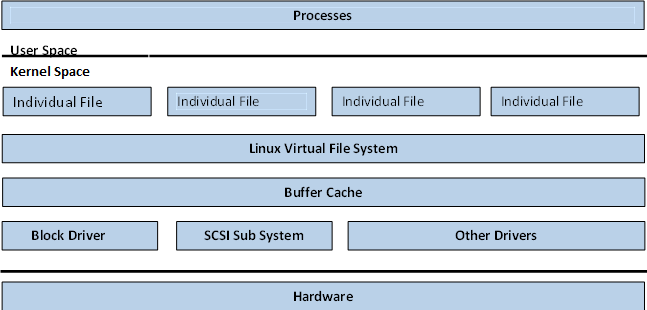
\includegraphics[scale=.9]
{fig2}

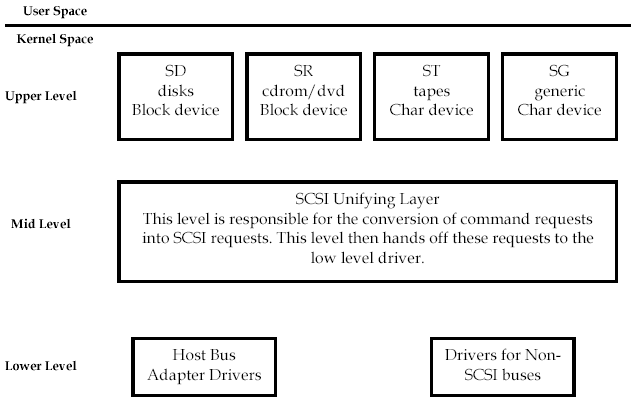
\includegraphics[scale=.9]
{fig3}


The SCSI subsystem in Linux consists of three layers namely Upper Level (ULD), Mid Level (SML) and Low Level (LLD).  The SCSI subsystem uses a three layer design with upper, mid, and low level layers. Every operation involving the SCSI subsystem (such as reading a sector from a disk) uses one driver at each of the 3 levels: one upper level driver, one lower level driver and the SCSI midlevel.\\

The SCSI upper level provides the interface between user space and the kernel, in the form of block and char device nodes for I/O and IOCTL. The low level contains drivers for specific hardware devices. In between is the SCSI midlevel, analogous to a network routing layer such as the IPv4 stack. \\

The SCSI midlevel routes a packet based data protocol between the upper levels device nodes and the corresponding devices in the lower level. It manages command queues, provides error handling and power management functions, and responds to I/O control (IOCTL) requests. The upper level and midlevel drivers are developed by Linux kernel SCSI developers.  There will be at least one type of upper level driver for a type of SCSI device. For example the SD driver handles all disk drives and the ST driver handles tape devices and similarly other upper level driver handles a particular type of device. The midlevel driver named scsi\_mod handles the entire house keeping activities like timing the SCSI requests and handling errors etc and it is a core for the SCSI driver model in Linux.  The midlevel driver also is maintained by Linux SCSI developers. \\

The low level drivers are the hardware specific driver and they translate the SCSI commands sent by the midlevel into the commands which can be understood by the hardware.  Hence the low level drivers are usually developed and maintained by hardware manufacturing companies. The Linux kernel community does rigorous code reviews before accepting driver code submission from the hardware vendor into kernel source tree.  \\

Considering the above, it will require a humongous work to develop one generic common unit testing frame work for all Linux kernel modules. Hence we decided to approach the problem in piece meal fashion.\\

As mentioned above, the SCSI subsystem is a major class of device drivers of the Linux operating system. It provides support for peripheral devices that support the SCSI interface, such as high performance hard drives. The code for the SCSI subsystem can be found in the ``drivers/scsi" directory of the source code distribution. SCSI support has been present in Linux since the first official release of the kernel in 1994. Like the rest of the kernel, the SCSI drivers are open source. However most of the low level drivers have been developed and then donated by the companies that developed the SCSI controllers themselves. That is, unlike much of the core of the Linux kernel, the original development of most of the low level driver code was performed within a company by full time developers, and not by the open source community. \\

One noteworthy feature of the SCSI subsystem is that it is designed and implemented as a strict three level architecture: the top and middle levels provide a set of unified and consistent commands for the kernel to control various drivers while the low-level drivers are concrete implementations of this functionality peculiar to the specifics of the particular hardware. Abstractly, the low-level drivers all implement the same functionality, such as hardware initialization, I/O handling, and error checking; they interact with the rest of the operating system only through the upper two levels.\\

The controlled interfaces between the low level and midlevel and most common functionalities between various low level drivers make low level driver (LLD) as in ideal candidate for unit testing using a generic unit test tool.  The unit testing of LLD also has similar limitation of other kernel modules.  Today to test a LLD, the test cases are executed from user space through the generic application interface available and requires whole stack. The LLD are developed by hardware vendors and testing of the LLD are typically done after integrating the driver into the complete stack and by running applications to execute the LLD functionalities from user space.  The application calls has to pass through all the layers above LLD to test a particular functionality of LLD this is an unnecessary overhead and nullifies the whole purpose of unit level testing. If there is any failure, lot of debug effort is required to isolate a fault at unit level.  Also testing a LLD interface thoroughly is not possible today as it is not standalone. Certain functionalities cannot be tested due to restrictions imposed by the upper levels.  For example there is an interface implemented by LLD named \textit{queuecommand}, the \textit{queuecommand} interface of an individual LLD will be invoked by the midlevel when it wants to send a new command to a hard drive. The LLD is expected to validate the command and return error when the command is sent to an unknown device.  But due to the reason that SML keeps track of only known devices, that condition can never be tested through SML.  If in future if the SML send a command to unknown device if LLD cannot capture that and return error it will results in failure of LLD.  \\

The Linux community recognizes the need for unit test tool for LLD as over the last 20 years, the    LLD code base is increased from 0 to 500 K but there is no available test tool for validating LLD before acceptance into kernel source tree. \\

Hence we are motivated to 
\begin{enumerate}
\item Port an application level unit test tool for C to kernel. 
\item Develop a Kernel module and associated applications to commonly test various interfaces of LLD by utilizing the unit test tools ported to kernel.
\end{enumerate}

Unit testing of LLD requires two different levels of testing.  One is to test the higher level interaction of the LLD (with SML or ULD) and the other is testing the hardware interaction.  Writing a common unit test module to hardware level is not really possible as the hardware interaction is in general is through proprietary interfaces provided by hardware vendors. So we will be limiting our efforts to unit testing of higher level interaction interfacing of LLD.\\




 % \input{Impact}
 % \input{Discussion} 
  % Research question 2 is not reviewed!
\vspace{3 mm}
\section{Proposed work}\vspace{3 mm}

As stated above, the low level drivers are provided by many third party hardware vendors so if we develop a common unit testing tool then it will benefit both Linux community and the hardware vendors by helping to harness the low level drivers and increasing the overall quality of LLDs. Hence we propose to develop one such tool which can exercise various interfaces provided by LLD with the purpose of identifying issues at unit level.  This tool will exercise the different units/interfaces of LLD with varying input combinations and make sure the LLD interfaces behave as defined by Linux SCSI community and as expected by the SML. \\

The low level driver interacts with SML in two ways.  The LLD invokes certain functions of SML and in addition it provides set of interfaces it exposes to SML through a registration process.  The picture shown below depicts the high level interactions between the LLD and SML. \\

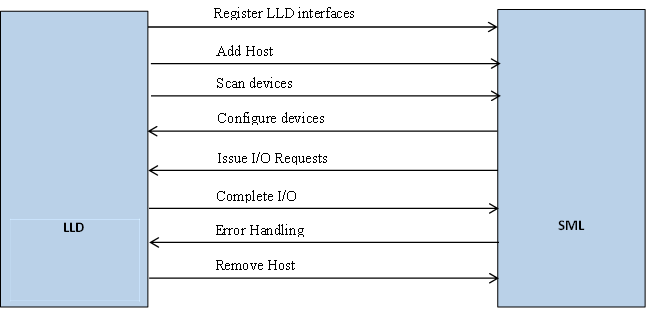
\includegraphics[scale=1]
{fig5}

We propose to introduce a new kernel module named LLD Tester (LLDT) which will be layered between LLD and SML and trap all the communication between LLD and SML. The LLDT module will then interact with SML.  By doing so, the LLDT will get control of the interfaces of LLD and can introduce new test cases or test data and execute LLD in unit test mode. 

The LLD module will also contain either CUnit/CuTest ported to kernel level and will utilize the interfaces of the Unit Test tool for test case management, test suit creation and test status update.  Since there is no way to ASSERT in kernel module the test status needs to be logged into the system logger files.

In addition to the LLD tester kernel module a user level helper application will also be developed. It will provide the context for the kernel module to run the test cases, help in configuring the test cases to run and collect test execution status.  

For introducing the LLDT, the LLD needs to be modified to a small extent, there will be a function mapper file provided by LLDT and the LLD needs to be compiled with the function mapper so that the LLD’s SML interaction can be directed to LLDT. 

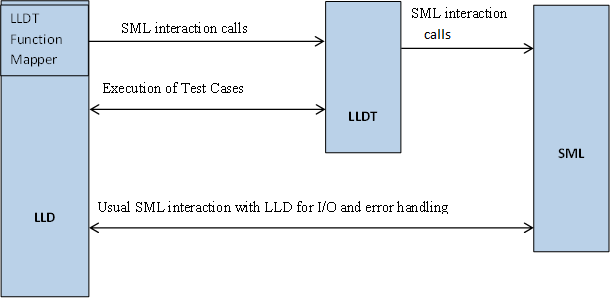
\includegraphics[scale=1]
{fig6}

The picture below shows the components of LLDT. \\

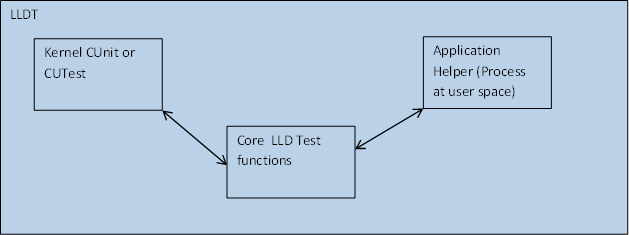
\includegraphics[scale=1]
{fig7} %6
  \section{Evaluation}\vspace{3 mm}

\par The scsi\_debug driver is sample LLD without needing any actual hardware.  The LLDT will be validated with the scsi\_debug driver initially.  The LLDT functionality will be evaluated with the scsi\_debug by creating one or more positive/negative test cases for the scsi\_debug interfaces.  The test execution and defect details if any will be captured.  Once the LLDT is tested with confidence the tests will be executed on one or more real drivers. Obtaining actual SCSI host controllers for this testing is time and cost prone, hence the virtual machines which expose one or more host controllers will be used and the tests will be executed on the drivers for the virtual machine exposed pseudo host controllers.  \\

The test results and defect if any will be shared with the owners of the particular driver  or through  Linux SCSI driver development community and based on their acceptance of the defect the efficiency of the LLDT can be measured. \\

There is no standard test suite for validating of Linux kernel modules especially the LLD.  So using the LLD tester we need to write test cases for various interfaces of LLD and make sure that the test cases are effective by adding mutants in the LLD interface and confirming the test case identifies the mutant.\\

For example, if you take queuecommand interface, the expected return value of the interface for successful queuing of I/O request is 0 and all other failure cases the queue command has to return non zero values. We might write a test case to validate whether a wrong invocation of queuecommand will properly return error value but to validate whether our test properly reports the error we need to modify the queuecommand interface under test to return 0 for failures and make sure the test case prints the failure properly.\\

\subsection{Threats to Validity}

\begin{sloppypar}For generating mutants, we used the mutation tool MiLu. We tried it on scsi\_debug.c which is a sample driver which will be used with LLDT.  We just did try to create a mutant for the function ``scsi\_debug\_queuecommand\_lck”.\\
\end{sloppypar}

This did work partially and the problem is the mutated code was not having some important data structure pointers and initializations.  The first thing we noticed was that MiLu requires the source file to be run with for example ``gcc -E". This is stated in the information about MiLu. This means that the source file needs to be run through the preprocessor before MiLu is able to mutate the file but the problem is we are compiling the kernel code and we do not have all the headers require for generic preprocessing to be successful.  We further need to explore how to overcome this though we have a limited set of tools available for C, there seems to be no tool to mutate the kernel code.


   
\section{Completed work} \vspace{3 mm}

The deliverables of this project are:

\begin{enumerate}
\item A kernel header file for LLD to consume and use as a plugin to interact with LLD tester
\item A LLD tester kernel module code which will have CUTest ported to Linux kernel as unit test framework and in addition will have kernel module with generic test cases common for any LLD.
\item A user level application to configure the test cases, initiate test run and collect the test execution reports
\item A user guide to how to use the generic test cases and extend the LLD tester for a specific functionality of LLD.
\item Evaluation reports of the execution of generic test cases using LLD tester against two or more LLD, mutation information and efficiency of test cases by number of mutant identified by the test cases. 

\end{enumerate} %3.5
    
% check if the in-text citations are good. 
 \section{Related work}\vspace{3 mm}

There are numerous Unit testing frameworks and tools available for various different languages.  The \url{http://en.wikipedia.org/wiki/List_of_unit_testing_frameworks} lists majority of available unit testing frameworks.  \\
Most of current research is happening on unit testing framework for object oriented languages especially Java.  The Junit (\url{http://junit.org/}) is most famous framework available for unit testing Java based object oriented code and researches are happening in the direction of optimizing test suite based on automated unit testing of Java code using Junit.\\
\begin{sloppypar}
(\url{http://www.ist.tugraz.at/teaching/pub/Main/QS/cheon-leavens04_jmlunit.pdf}) and unit testing concurrent programs using Junit (\url{http://www.cs.rice.edu/~javaplt/drjava/papers/PPPJ2009-Ricken-ConcJUnit.pdf}) .\\
\end{sloppypar}
There are some existing frameworks for unit testing C code, but there are no noticeable researches which we are aware in unit testing for C code.  One of the famous available unit testing frameworks for C is Cunit (\url{http://cunit.sourceforge.net/}) . The CuTest is a simple and lightweight framework (\url{http://cutest.sourceforge.net/}).   However the existing majority of frameworks are available in user space and good in unit testing user level programs but not kernel code.   \\
The kernel itself and its parts are tested prior to the release, but these tests cover only the basic functionality. There are some testing systems which perform testing of Linux Kernel:\\

The Linux Test Project (LTP) delivers test suites to the open source community that validates the reliability and stability of Linux. The LTP test suite contains a collection of tools for testing the Linux kernel and related features. \url{https://github.com/linux-test-project/ltp} \\

Autotest -- a framework for fully automated testing. It is designed primarily to test the Linux kernel, though it is useful for many other purposes such as qualifying new hardware, virtualization testing, and other general user space program testing under Linux platforms. It's an open-source project under the GPL and is used and developed by a number of organizations, including Google, IBM, Red Hat, and many others. \url{http://autotest.kernel.org} \\

Also there are certification systems developed by some major GNU/Linux distribution companies. These systems usually check complete GNU/Linux distributions for compatibility with hardware. There are certification systems developed by Novell, Red Hat, Oracle, Canonical, Google.\\

There are also systems for dynamic analysis of Linux kernel: \\

Kmemleak is a memory leak detector included in the Linux kernel. It provides a way of detecting possible kernel memory leaks in a way similar to a tracing garbage collector with the difference that the orphan objects are not freed but only reported via /sys/kernel/debug/kmemleak. \\

Kmemcheck traps every read and write to memory that was allocated dynamically (i.e. with kmalloc()). If a memory address is read that has not previously been written to, a message is printed to the kernel log. Also is a part of Linux Kernel. \\

Fault Injection Framework (included in Linux kernel) allows for infusing errors and exceptions into an application's logic to achieve a higher coverage and fault tolerance of the system. \\

Though there are complex test suits like LTP, Autotest are available, there are thousands of combination of devices, kernels, device drivers possible for testing and testing everything is beyond the scope of a centralized automatic test suite, hence majority of Linux kernel testing is dependent on developers who develop a particular kernel module or device drivers.   \\

As stated previously the LLD are developed by developers employed in hardware vendor organization and dedicating their time in validating using complex framework like LTP is highly impossible and the LLD tester is light weight and specifically targeted for LLD.\\



 %1.5
    
\section{Tasks and Timeline}\vspace{3 mm}


  \par 2/28:  Complete background and a basic design of the project and submit proposal. \\

3/23:  Port the CuTest to kernel, develop the kernel module and user space application, develop and the generic test cases. \\

3/31:  Validate the generic LLD test cases against the sample LLD. \\

4/5:  Fix any issues found in the testing with sample LLD. \\

4/15: Validate the generic LLD test cases against the an virtual hardware driver. \\

4/20:  Create user guide and evaluation reports. \\
 %0.5
    
\section{Conclusion} \vspace{3 mm}

TBD
  %\input{appendix} 



%   ==========================================================================
%   Wrap up the document with the Bibliography (looks for the specified .bib)
%   ==========================================================================
\makebibliography{sources}
\end{document}
